% Measuring and Exploiting Near-Duplicate Instruction Sequences in Executables
% Compile: pdflatex neardup; bibtex neardup; pdflatex neardup; pdflatex neardup
\documentclass[conference]{IEEEtran}
\IEEEoverridecommandlockouts
\usepackage{cite}
\usepackage{amsmath,amssymb}
\usepackage{graphicx}
\usepackage{booktabs}
\usepackage{array}
\usepackage{xcolor}
\usepackage{microtype}
\usepackage{url}
\usepackage{listings}
\usepackage{hyperref}
\hypersetup{colorlinks=true,linkcolor=blue!60!black,citecolor=green!40!black,urlcolor=blue!70!black}
\newcommand{\tu}{\texttt{dmmeta\_gen}}
\newcommand{\amc}{\texttt{amc}}
\lstset{basicstyle=\ttfamily\scriptsize,breaklines=true,columns=fullflexible,
        keepspaces=true,xleftmargin=4pt,aboveskip=3pt,belowskip=3pt}

\begin{document}

\title{Measuring and Exploiting Near-Duplicate\\Instruction Sequences in Executables}

\author{%
  \IEEEauthorblockN{Ara Aslyan}
  \IEEEauthorblockA{Strike Technologies, New York, USA\\
                    \texttt{aaslyan@striketechnologies.com}}
  \and
  \IEEEauthorblockN{Ashot Harutyunyan}
  \IEEEauthorblockA{Yerevan State University, Machine Learning Lab, and\\
                    Institute for Informatics and Automation Problems, Armenia\\
                    \texttt{harutyunyan.ashot@ysu.am}}
}
\maketitle

\begin{abstract}
Compiled binaries, especially generated ones, can contain large amounts of
duplicate machine code, but the mechanisms deployed to remove it---linker
identical-code folding (ICF), GCC \texttt{-fipa-icf}, and the LLVM
\emph{MachineOutliner}---primarily exploit byte- or register-identical code
and cannot parameterize operand-differing near-duplicates. We show empirically
that the dominant duplication in real, production-optimized binaries is
\emph{near}-duplicate: functions with the same instruction skeleton that
differ only in operands, registers, or small blocks. On a code-generated
C\texttt{++} toolkit, $33$--$39\%$ of functions in a binary belong to
near-duplicate families. On the same generated translation unit, the LLVM
MachineOutliner removes $3.87\%$ at \texttt{-O3} and $0\%$ at \texttt{-Oz},
whereas a parameterizing source-level merge of one family removes
$22.7\%$---roughly $6\times$ more and additive to the outliner. We contribute
(i)~a measurement of how much near-duplicate code real binaries ship and of
what kind; (ii)~a document-frequency discriminator that separates likely
copy-paste from statically-linked library reuse without source; (iii)~a
profitability model (interface width $\times$ repetition $\times$ hotness)
deciding which merges pay; (iv)~a recursive, \emph{fuzzy-interface}
formulation that decomposes near-duplicate regions into a shared skeleton and
reusable outlined ``holes''; and (v)~a realized, behavior-preserving
transformation that reduces the binary's code section by $2.81\%$ from a
single family. Our finding is not a better outliner but a diagnosis:
production tool-chains leave most operand-differing near-duplication on the
table, and for code-generated software the right place to remove it is the
generator.
\end{abstract}

\begin{IEEEkeywords}
binary analysis, code size, function merging, outlining, code clones,
code generation, sequence alignment
\end{IEEEkeywords}

\section{Introduction}
Code size is a first-order concern: it drives instruction-cache and iTLB
pressure, program load time, memory footprint on constrained devices, and
even attack surface. Tool-chains therefore deduplicate code aggressively.
Linkers fold byte-identical functions via identical-code folding (ICF); GCC's
\texttt{-fipa-icf} folds functions with identical bodies; and the LLVM
\emph{MachineOutliner} \cite{paquette2016outliner} extracts repeated identical
instruction sequences into shared procedures. A common property unites them:
they act on code that is \emph{exactly} identical (in bytes, in body, or in
register-precise instruction runs).

Real binaries, however, are dominated by code that is \emph{almost} the same.
Consider a routine emitted once per record type by a code generator: each copy
loads the same kind of field, calls the same kind of helper, and returns the
same way, differing only in a type tag, a string literal, a structure offset,
or which register the allocator happened to choose. After compilation these
become distinct functions with an identical instruction \emph{skeleton} and a
handful of differing operands. Exact folding cannot merge them---the bytes
differ---so every copy ships in the binary.

The remedy is well known in principle: merge the copies into one function and
pass the differences as parameters. \emph{Function Merging by Sequence
Alignment} \cite{rocha2019fmsa} and its faster successors
\cite{rocha2020hyfm,rocha2021f3m} do exactly this---align two functions and
insert parameters or selects for the mismatches. But these are research passes
and are not enabled in production \texttt{-O2}/\texttt{-O3}. The mechanism
exists; whether it is reaching real binaries is a separate, empirical
question.

That is the question this paper answers: \emph{how much near-duplicate code do
real, production-optimized binaries actually ship, what kind is it, and is it
worth merging?} We treat it as a measurement and diagnosis problem rather than
as a new optimizer. Working from the opcode (mnemonic) stream recovered by
disassembly, we detect near-duplicate regions with sequence alignment,
separate likely copy-paste from library reuse using document frequency,
classify duplication into a small taxonomy, quantify how much each deployed
mechanism leaves behind, and finally realize a behavior-preserving
transformation to confirm the recoverable size on a real binary and to compare
head-to-head against the production outliner.

\textbf{Contributions.} This paper contributes:
(i)~a measurement of near-duplicate machine code in real optimized binaries
and a three-tier taxonomy of duplicate structure
(Sec.~\ref{sec:method},~\ref{sec:prevalence});
(ii)~a document-frequency discriminator that separates local duplication from
statically-linked library/runtime reuse without source (Sec.~\ref{sec:detect});
(iii)~a profitability and feasibility model based on liveness-derived interface
width, repetition count, and hotness (Sec.~\ref{sec:profit});
(iv)~a recursive fuzzy-interface formulation that decomposes near-duplicate
regions into skeletons and reusable holes (Sec.~\ref{sec:recursive}); and
(v)~a realized, behavior-preserving source-level transformation that reduces a
production binary's code section by $2.81\%$ from one generated family and
exposes a ${\approx}6\times$ gap over LLVM MachineOutliner on the same code
(Sec.~\ref{sec:realized}).

\section{Background and Related Work}
\textbf{Exact deduplication.} ICF (in \texttt{gold}/\texttt{lld}) and GCC
\texttt{-fipa-icf} fold byte- or body-identical functions; \texttt{-fipa-icf}
is on by default at \texttt{-O2}. The LLVM MachineOutliner
\cite{paquette2016outliner} scans the post-register-allocation instruction
stream for repeated identical sequences and outlines them; LLVM
\texttt{MergeFunctions} \cite{llvm_mergefunctions} merges functions that are
identical after a structural normalization. All require identical or
structurally identical instruction sequences and do not turn operand
differences into explicit parameters---which, as we show, is precisely where
most real near-duplication lives.

\textbf{Parameterizing merge.} Function Merging by Sequence Alignment
\cite{rocha2019fmsa} aligns two functions' instruction sequences, keeps the
matched instructions shared, and inserts parameters and a selector for the
mismatches; HyFM \cite{rocha2020hyfm} and F3M \cite{rocha2021f3m} reduce its
cost with locality-sensitive hashing of function fingerprints. This line
establishes the \emph{mechanism} we rely on. It does not, however, measure how
much exploitable near-duplication ships in real binaries, separate copy-paste
from library reuse, target code generators, or formulate recursive
hole-sharing---our contributions. We use the same alignment primitive
\cite{smithwaterman1981} as an analysis tool.

\textbf{Correctness.} Translation validation \cite{lee2018alive2} and verified
compilation \cite{leroy2009compcert} frame how to prove such transformations
equivalence-preserving. We adopt per-instance validation, observing that our
feasibility analysis already discharges the central proof obligation.

\textbf{Opcode statistics and binary similarity.} Opcode distributions have
been used for malware detection and cross-domain sequence analysis
\cite{bilar2007opcodes,gan2009statistical}; learned instruction embeddings and
function-similarity systems \cite{li2021palmtree,marcelli2022machine} and the
``naturalness'' of software \cite{hindle2012naturalness} establish that
assembly is statistically regular. We turn that regularity toward a
size-optimization diagnosis rather than classification or search.

\section{Method}
\label{sec:method}
\textbf{Extraction.} We disassemble with \texttt{objdump} and retain the
mnemonic-only opcode stream per function, $s=(o_1,\dots,o_N)$. Dropping
operands erases register- and immediate-level noise, so two copies differing
only in operands become \emph{identical} opcode streams and align exactly,
while genuinely different code remains distinguishable.

\textbf{Candidate generation and refinement.} For scalability we shingle each
function into opcode $k$-grams and index them with MinHash$+$LSH
\cite{broder1997minhash}; candidate pairs are refined with Smith--Waterman
local alignment \cite{smithwaterman1981}, and families are connected
components of the resulting similarity graph.

\textbf{Taxonomy.} We classify duplication by \emph{what differs} between
family members:
\emph{Tier~1}---byte-identical (linker-foldable);
\emph{Tier~2}---opcode-identical, operands differ (mergeable by promoting the
differing operands to \emph{value} parameters);
\emph{Tier~3}---near-duplicate, whole blocks differ (mergeable into a shared
\emph{skeleton} plus \emph{code} parameters, i.e.\ outlined holes).
Orthogonally, by document frequency across a corpus, a region is
library/runtime (high frequency), generator-induced, or copy-paste-like (low
frequency).

\textbf{Operand parameterization (Tier~2).} For an opcode-identical family we
align members position-by-position and, at each position, compare operands.
Positions whose operands are constant across all members remain in the body;
positions that vary become parameter candidates. Crucially, many mechanically
varying operands \emph{covary}: e.g.\ for a $77$-member accessor family in our
subject, $13$ varying operand slots collapse to only $4$ independent
parameters---a descriptor pointer driving $10$ slots, two small immediates,
and one callee---because slots that take a distinct value per member induce the
same member partition and are therefore driven by a single underlying
parameter.

\textbf{Skeleton/holes decomposition (Tier~3).} For a Tier-3 family we star-align
members to the longest member; conserved columns form the \emph{skeleton} and
maximal runs of divergent columns are \emph{holes}. For each hole we compute
its register/flags interface by local liveness on the reference function:
\emph{inputs} are upward-exposed uses (values read before being written inside
the hole) and \emph{outputs} are hole-defined values read after the hole.
Fig.~\ref{fig:align} illustrates the decomposition on two real functions: the
MATCH columns (identical instructions, operands included) are the skeleton and
the DIFFER columns are holes, supplied per member as parameters. The skeleton
is identical across members by construction, so instantiating it with a
member's arguments reproduces that member exactly; correctness follows from
this rather than from any approximation (Sec.~\ref{sec:correct}).

\begin{figure}[t]\centering
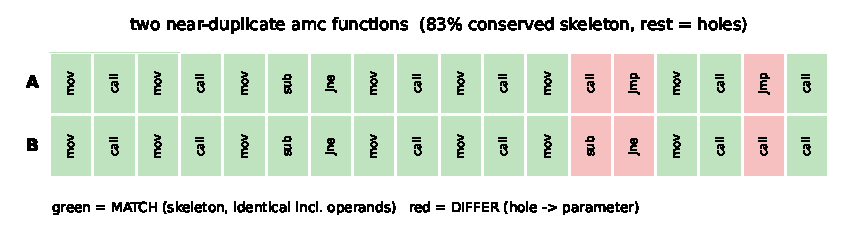
\includegraphics[width=\columnwidth]{fig_alignment.pdf}
\caption{Skeleton/holes on two real near-duplicate \amc{} functions. Each
column is an aligned position; green columns MATCH (the shared skeleton,
identical including operands), red columns DIFFER (holes, supplied per member
as parameters). Here $83\%$ of columns are skeleton; the rest are cut into
holes.}
\label{fig:align}
\end{figure}

\section{Detection and Discrimination}
\label{sec:detect}
\textbf{Detection (controlled ground truth).} We compiled a C source
containing a function together with a verbatim copy, an edited copy, and a
register-reallocated copy, plus a hard negative (a different algorithm with the
same loop shape). At \texttt{-O2} opcode alignment separates every copy pair
from non-copies (similarity $\geq0.63$ vs $\leq0.20$ for gcc; $\geq0.27$ vs
$\leq0.11$ for clang) and detects $6/6$ copies including the edited and
reallocated ones, whereas exact opcode-string matching detects only $3/6$. Two
limits emerged: at \texttt{-O0} generic stack scaffolding inflates the
similarity of unrelated functions and confounds detection, and cross-compiler
similarity is low ($0.03$--$0.27$). Opcode-level detection is therefore
reliable \emph{within one build configuration}---the realistic case for
copy-paste inside one project built one way.

\textbf{Discrimination.} Two binaries that statically link the same library
share a large block of \emph{identical} code, indistinguishable from
copy-paste by similarity score alone. Document frequency (DF) separates them
(Fig.~\ref{fig:idf}). Over a $27$-binary \texttt{/usr/bin} corpus
($394{,}358$ distinct $12$-grams, with only a tiny universal core), an
injected ground-truth copy-paste appears in exactly its two binaries
($63$ exclusive shingles), real shared \texttt{gnulib} code between
\texttt{md5sum} and \texttt{sha256sum} appears as $958$ exclusive shingles,
and an unrelated pair shares only $11$ (the noise floor). Library reuse is
high-DF; copy-paste is low-DF; similarity score is the wrong axis,
\emph{frequency} is the right one.

\begin{figure}[t]\centering
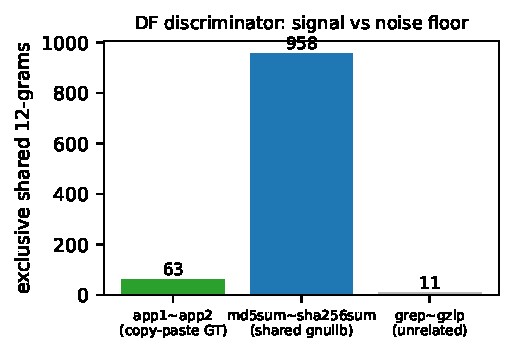
\includegraphics[width=\columnwidth]{fig_idf.pdf}
\caption{Document-frequency discriminator. Shingles shared \emph{exclusively}
by a binary pair: injected copy-paste and shared library both ``light up''
well above the unrelated-pair noise floor; document frequency across the
corpus (not shown here) is what separates the first two.}
\label{fig:idf}
\end{figure}

\section{Prevalence and Recoverable Opportunity}
\label{sec:prevalence}
We study a non-stripped, code-generated C\texttt{++} toolkit (OpenACR), whose
\amc{} generator emits per-type accessor functions; this makes it an ideal,
ground-truthed subject for generator-induced duplication.

\begin{table}[t]\centering
\caption{Near-duplicate function prevalence (opcode-only, functions
$\geq12$ instr., Jaccard $\geq0.85$).}
\label{tab:prev}
\begin{tabular}{@{}lccc@{}}\toprule
\textbf{Binary} & \textbf{Functions} & \textbf{Opcode-identical} & \textbf{Near-dup families}\\\midrule
\amc      & 2022 & 32.9\% & 38.9\%\\
atf\_unit & 1318 & 29.1\% & 33.2\%\\
aqlite    & 1624 & 5.4\%  & 6.9\%\\\bottomrule
\end{tabular}
\end{table}

\textbf{Intra-binary.} Table~\ref{tab:prev} and Fig.~\ref{fig:prev} show that
$33$--$39\%$ of functions in generated binaries belong to near-duplicate
families. \texttt{aqlite}, which is mostly hand-written external SQLite code,
is an order of magnitude lower, so the near-duplicate rate tracks how much of a
binary is machine-generated rather than being an artifact of our method. The
analysis is implemented as a single reusable tool that takes arbitrary
binaries; run across $42$ executables, opcode-identical prevalence ranges from
$5.4\%$ (hand-written \texttt{aqlite}) to $32.6\%$ (\amc), with mergeable
opportunity from a few KB up to $113$\,KB per binary.

\begin{figure}[t]\centering
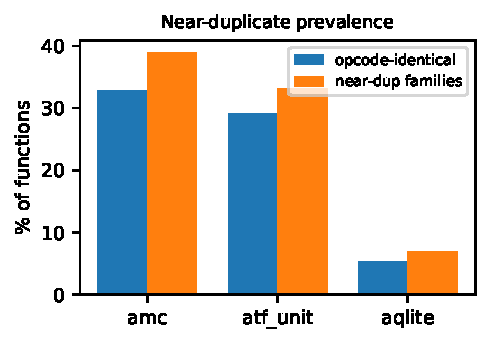
\includegraphics[width=\columnwidth]{fig_prev.pdf}
\caption{Near-duplicate prevalence per binary. The rate tracks the fraction of
each binary that is code-generated (\texttt{aqlite} is mostly hand-written).}
\label{fig:prev}
\end{figure}

\textbf{Cross-binary.} Across $44$ executables, of $6{,}189$ distinct function
signatures, $5{,}291$ ($85\%$) are unique to a single binary, $413$ are shared
by $2$--$3$ binaries (copy-paste / narrow-sharing candidates), and $148$
appear in \emph{all} $44$---the statically-linked runtime
(Fig.~\ref{fig:df}). DF cleanly stratifies the corpus into tool-specific code,
narrowly-shared code, and ubiquitous runtime.

\begin{figure}[t]\centering
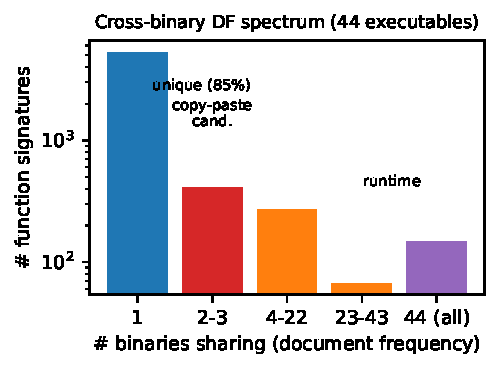
\includegraphics[width=\columnwidth]{fig_df.pdf}
\caption{Cross-binary document-frequency spectrum over $44$ executables (log
scale). Most code is unique; a thin band is narrowly shared (copy-paste
candidates); a small core is the runtime linked into every tool.}
\label{fig:df}
\end{figure}

\textbf{What exact mechanisms leave behind.} On \amc{}, $608$ functions
($31\%$) are opcode-identical duplicates, yet only $3$ are byte-identical, so
ICF and \texttt{-fipa-icf} reach about $0.1\%$ of \texttt{.text}. Promoting
operands to parameters (Tier~2) instead exposes an estimated $10.6\%$
(${\approx}112$\,KB). On a single generated translation unit, three accessor
families (\texttt{ReadStrptrMaybe}, \texttt{ReadFieldMaybe}, and getters)
account for ${\approx}106$\,KB of near-duplicate code.

\section{Profitability and Feasibility}
\label{sec:profit}
Merging pays only when the shared body dominates the per-call overhead. For a
family of $N$ members, a hole of size $s$ instructions, and a per-call-site
interface overhead $o\approx(\#\text{inputs}+\#\text{outputs}+2)$, the net
saving is
\begin{equation}
\Delta = (N-1)\,s \; - \; N\,o .
\end{equation}
Interface width is computed by liveness: a hole is a clean outline target when
few values cross its boundary. The same quantity is a \emph{correctness} side
condition---the interface must capture \emph{all} crossing values, including
processor flags---so the feasibility analysis doubles as a soundness check
(Sec.~\ref{sec:correct}).

Across $40$ Tier-3 families in \amc{}, the largest (a $15$-member insert
routine) is $72\%$ conserved skeleton with three sizeable holes; over all
families the holes carry $11{,}204$ instructions of reduction that is
unreachable by exact or value-only merge. Of $84$ large holes, $92\%$ have a
narrow interface; under the net-saving model $61\%$ ($51/84$) are profitable.
Notably, $4$ of $7$ \emph{wide}-interface holes remain profitable because high
repetition amortizes a wide interface (e.g.\ $N{=}12$, $68$ instructions,
$5$ inputs/$4$ outputs $\Rightarrow$ net $+616$ instructions). Interface width
alone is the wrong gate; net saving---width \emph{times} repetition---is the
right one, modulated by hotness (cold, repetitive, wide holes still merge
well; hot inner loops prefer inlining).

Feasibility is governed by a small set of explicit parameters---minimum hole
size, maximum tolerated interface width, the overhead model, and minimum
repetition---rather than fixed constants. Fig.~\ref{fig:sens} sweeps the two
principal ones. The maximum interface width is the dominant lever: relaxing it
from $\leq4$ to $\leq6$ crossing values more than doubles the recoverable
instructions, whereas raising the hole-size floor from $2$ to $12$ costs only
${\approx}6\%$. The binding constraint on profitable merging is the data-flow
interface, not the size of the differing block.

\begin{figure}[t]\centering
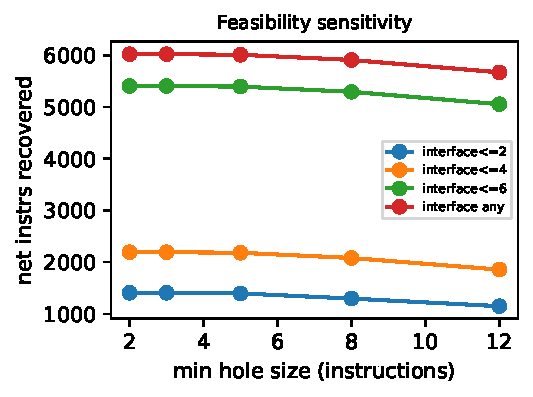
\includegraphics[width=\columnwidth]{fig_sensitivity.pdf}
\caption{Feasibility sensitivity. Recoverable net instructions versus minimum
hole size and maximum interface width: interface width dominates; the
hole-size floor is secondary.}
\label{fig:sens}
\end{figure}

\section{Recursive Fuzzy-Interface Merging}
\label{sec:recursive}
A skeleton/holes decomposition shares the skeleton once. But holes are
themselves code fragments that recur \emph{across} families, so we recurse:
pool all holes and deduplicate them. Once a hole is an outlined function rather
than an inlined fragment, register naming becomes irrelevant---the interface is
a \emph{signature shape}---so two holes that differ only by register
allocation are the same function. We therefore cluster holes by \emph{fuzzy
interface}: holes whose opcode content aligns ($\geq0.85$) and whose interfaces
differ by at most one input/output are unified, widening the shared signature
(and ignoring the surplus argument) where needed.

The effect is decisive. Exact hole-sharing is negligible: $7$ holes in $3$
clusters, $14$ instructions saved. Fuzzy-interface clustering collapses the
$84$ holes to $55$ clusters and saves $1{,}062$ second-order
instructions---$75\times$ the exact approach---with $12$ of $13$ unifying
clusters \emph{requiring} interface widening. Recursion composes because
observational equivalence is a congruence; widening additionally needs a
dead-argument soundness lemma (the surplus parameter must be unused in the
narrower instantiation). The fuzzy/widening step, not exact matching, is what
unlocks second-order reuse.

\section{Realized Transformation and Baseline Comparison}
\label{sec:realized}
We realize the Tier-2 merge on real \amc{} source. The
\texttt{ReadStrptrMaybe} family is maximally regular: each member differs only
in its type, two string literals, and a per-type callee. A source rewrite
replaces each member with a thin thunk to one type-erased shared helper:

\begin{lstlisting}
static bool Rsm_shared(void* p, strptr in,
   const char* lc, const char* uc, RsmRF rf){
 bool r=true;
 r = StripTypeTag(in,lc)||StripTypeTag(in,uc);
 ind_beg(Attr_curs,a,in){ r=r&&rf(p,a.name,a.value);}ind_end;
 return r; }
// per type T:
bool T_ReadStrptrMaybe(T& parent, strptr in){
 return Rsm_shared(&parent,in,"t.lc","t.uc",(RsmRF)T_ReadFieldMaybe); }
\end{lstlisting}

\noindent The type-erased function-pointer cast is legal under the project's
own \texttt{-Wno-cast-function-type}. We reproduce the exact production build
command (\texttt{gcc -O3}); our baseline object matches the shipped object
byte-for-byte ($159{,}980$\,B \texttt{.text}), confirming a faithful
reproduction. Because MachineOutliner is an LLVM facility, the comparison in
Table~\ref{tab:realized} is run under \texttt{clang}, and its percentages are
over the \emph{translation unit's} \texttt{.text} (clang's \texttt{-O3}
baseline for this unit is $110{,}111$\,B); the whole-binary figure below is
over \amc{}'s \texttt{.text}.

\begin{table}[t]\centering
\caption{Realized code-size reduction and comparison to production mechanisms
(real \tu, clang \texttt{-O3} unless noted).}
\label{tab:realized}
\begin{tabular}{@{}lcc@{}}\toprule
\textbf{Configuration} & \textbf{.text (B)} & \textbf{removed}\\\midrule
baseline (clang -O3)                 & 110{,}111 & ---\\
+ LLVM MachineOutliner               & 105{,}854 & 3.87\%\\
\textbf{our merge (one family)}      & 85{,}141  & \textbf{22.68\%}\\
merge + MachineOutliner              & 80{,}996  & 26.45\%\\\midrule
clang -Oz, no outliner               & 95{,}910  & ---\\
clang -Oz, + MachineOutliner         & 95{,}910  & 0.00\%\\
clang -Oz, our merge + outliner      & 77{,}244  & 19.46\%\\\bottomrule
\end{tabular}
\end{table}

\textbf{Comparison.} On identical real code (Table~\ref{tab:realized},
Fig.~\ref{fig:compare}), the LLVM MachineOutliner removes $3.87\%$ of the
translation unit at \texttt{-O3} and $0\%$ at \texttt{-Oz}: it folds
register-identical runs but cannot parameterize the differing operands. Our
merge of one family removes $22.68\%$ of the same translation unit
(${\approx}6\times$ more) and is \emph{additive} to the outliner ($26.45\%$
combined), since the two target different classes. We also tested the strongest
\emph{deployed} IR-level mechanism, LLVM \texttt{MergeFunctions} (run explicitly
via \texttt{opt}, as it is not in the default \texttt{-O2/-O3} pipeline): it
removes $7.89\%$ of the unit---more than the machine outliner, but still
${\approx}2.9\times$ less than our merge, because it folds structurally
identical functions yet does not parameterize differing constants or callees.
Across all three deployed layers---byte (ICF, ${\approx}0.1\%$), IR
(\texttt{MergeFunctions}, $7.89\%$), and machine (\texttt{MachineOutliner},
$3.87\%$)---operand-differing near-duplication is left largely unmerged. The shipped
binary, built with \texttt{gcc -O3} (\texttt{-fipa-icf} on by default), still
contained all $243$ family copies, corroborating that deployed exact folding
does not reach this class.

\begin{figure}[t]\centering
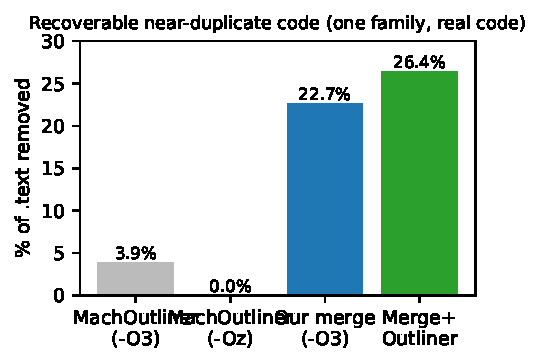
\includegraphics[width=\columnwidth]{fig_compare.pdf}
\caption{What each mechanism recovers on the same real code (one family). The
production outliner reaches $\leq3.87\%$; parameterizing merge reaches
$22.7\%$ and is additive to the outliner.}
\label{fig:compare}
\end{figure}

\textbf{Whole-binary, behavior-preserving.} Merging the family across all $10$
generated translation units and rebuilding \amc{} reduces its \texttt{.text}
from $1{,}637{,}878$ to $1{,}591{,}871$\,B ($-2.81\%$) from a \emph{single}
family. The build is clean under \texttt{-Werror}, a read-only query
(\texttt{acr ctype:\%}) produces byte-identical output ($1{,}419$ lines) before
and after, and the full \texttt{atf\_unit} suite shows \emph{no regressions}:
stock and merged builds both run $254$ tests with the same $6$ pre-existing
failures (unrelated to the merge), the only output differences being
nondeterministic temporary-file names and timing values. A controlled microbenchmark confirms the size/speed trade-off:
realistic $122$-byte accessors merge to $-30\%$ \texttt{.text} with identical
output at $+8\%$ runtime; the shared body must be marked \texttt{noinline} or
\texttt{-O2} re-inlines it and reverses the merge; and below a size threshold
(e.g.\ $55$-byte bodies) merging loses on both size and speed because overhead
exceeds the body.

\section{Correctness}
\label{sec:correct}
We claim no new theorem. Correctness here is the standard notion of
\emph{observational (behavioral) equivalence}, established by the usual
simulation argument from verified compilation \cite{leroy2009compcert} and
translation validation \cite{pnueli1998tv,lee2018alive2}: a relation pairs an
original machine state with a transformed state that agree on all live,
non-scratch locations, and each original step is matched while the relation is
preserved. What we provide is the \emph{specialization} of that argument to
skeleton/holes merging---a set of \emph{proof obligations}, each a restatement
of a well-known requirement:
(1)~\emph{skeleton identity}---conserved positions are syntactically identical
(by construction of the alignment);
(2)~\emph{pure operand substitution}---each operand promoted to a parameter is
bound at the call site to exactly its original value;
(3)~\emph{interface completeness}---each hole's interface captures every value
crossing its boundary (live-in/live-out registers, flags, memory), which is
precisely the live-variable analysis underlying procedural abstraction and
outlining \cite{cooper1999pa,debray2000compaction};
(4)~\emph{ABI/frame preservation}---caller/callee-saved registers, stack
alignment, and frame-relative access are preserved; and, for the recursive
fuzzy-interface step (Sec.~\ref{sec:recursive}),
(5)~\emph{dead-argument soundness}---when two holes are unified by widening to a
superset signature, the surplus parameter is unused in the instantiation that
did not require it.

\textbf{Completeness is correctness; width is profitability.} Obligation (3)
requires the interface be \emph{complete}, not narrow. The
maximum-interface-width parameter of Sec.~\ref{sec:profit}
(Fig.~\ref{fig:sens}) is a profitability filter, not a correctness condition:
widening the tolerated interface only adds parameters to an already-complete
interface, changing which merges pay but never their soundness. Our liveness
feasibility gate computes exactly the interface of obligation (3), so the same
analysis that scores profitability also discharges the central soundness
check---a hole that produces flags read after it but omits them from its
interface is an \emph{incorrect} merge, not merely an expensive one.

\textbf{Assurance in practice.} We discharge these obligations per instance
rather than once-and-for-all over a full x86 semantics: the realized merge
compiles under production \texttt{-Werror} flags, passes a differential test
on real data (identical query output), and introduces no regressions across the
full \texttt{atf\_unit} suite. A full per-instance SMT equivalence
check \cite{lee2018alive2} is future work, and recursion composes because
observational equivalence is a congruence. Obligation (4) is
platform-specific---our type-erased merge is sound on the x86-64 SysV ABI we
tested and would need re-checking on another ABI.

\section{Discussion}
The gap between deployed mechanisms and the available opportunity is
structural, not a tuning artifact: outlining and ICF require register/byte
identity, whereas the dominant near-duplication differs in operands. Three
deployment points are possible. A \emph{compiler pass} (as in
\cite{rocha2019fmsa}) is general but competes with mature infrastructure and
pays an indirect-call cost. \emph{Post-link} rewriting is hardest. For
code-generated software, the cheapest and safest point is the
\emph{generator}: emitting one parameterized helper removes the duplication at
the source, leaves the compiler free to inline where hot, and avoids the
indirect call entirely. This is why we frame the result as a diagnosis with an
actionable target rather than as another optimizer.

On the size/speed question, smaller code is not strictly a trade against
speed: for cold, scattered code---which generated accessors typically
are---reducing the footprint improves instruction-cache and iTLB behavior and
can be net-positive, while hot inner loops favor inlining. The hotness term in
the profitability model captures this, and the realized microbenchmark
($+8\%$ on a hot synthetic loop) bounds the worst case.

\section{Threats to Validity}
\emph{Construct.} Opcode normalization discards operands, so similarity reflects
structural rather than semantic equivalence; we therefore validate merges
behaviorally rather than claim semantic equivalence from the opcode stream
alone. \emph{Internal.} Most opportunity figures are estimated from
disassembly; one family in one binary is fully realized and behavior-checked,
and the comparison against MachineOutliner is measured on real code.
\emph{External.} Results are x86-64-specific and centered on one
code-generated subject plus a controlled corpus; \texttt{-O0} confounds
detection and cross-compiler detection is weak. \emph{Provenance.} From a
binary one cannot infer whether a near-duplicate arose from human copy-paste,
templates, macros, or a generator; we use ``copy-paste-like'' for low-DF
near-duplicates without asserting source-level cause.

\section{Conclusion}
Production-optimized binaries ship with substantial near-duplicate machine code
that deployed mechanisms do not remove: on real code the LLVM MachineOutliner
reaches $\leq3.87\%$ of one family (and $0\%$ in size mode), while a
parameterizing merge reaches $22.7\%$, additively. We measured how much such
code exists and of what kind, separated copy-paste from library reuse without
source, modeled when merging pays, gave a recursive fuzzy-interface
formulation that unlocks second-order reuse, and realized a behavior-preserving
$2.81\%$ whole-binary reduction from a single family. The actionable
conclusion is to remove generator-induced duplication in the generator. Future
work: realize Tier-3 families via data-driven dispatch, formal per-instance
validation, and multi-architecture, multi-tool-chain measurement.

\bibliographystyle{IEEEtran}
\bibliography{references}
\end{document}
